\chapter{Selection and Adversary Arguments}\label{Sec:Chapter:SelectionandAdversaryArguments}
\section{概述}
在这章中我们学习几个可以被归类到一个通用名字\emph{selection}的问题。找到
一个集合的中间元素是一个总所周知的例子。除了找到有效解决问题的算法,
我们还将找到这类问题的\emph{底限}。我们会介绍一种被称为adversary
arguments的广泛应用的技术来建立底限。

\subsection{Selection问题}
假设E是包含n个元素的数组,数组元素的关键字属于某个线型集合,令k是
的一个整数 $1\leq k \leq n$。selection问题是找到E中第k小的元素。
这样的元素叫做有\emph{rank k}。与我们学过的排序算法一样,我们将假定
唯一的操作是比较两个关键字(以及拷贝或是移动元素)。在这一章中关键字
和元素是一样的,因为我们注意的是关键字比较的次数,而且我们一般不
关心元素移动。还有,当关键字在一个数组中存放时,我们将使用位置
$1, \cdots, n$而不是$0, \cdots, n-1$以符合一般的rank术语,位置0只是
简单的放在那里不用。

在第一章中我们解决了一个$k=n$的selection问题,那个问题是简单的找到最大
的元素。我们考虑了一个最简单的算法做了n-1次关键字比较,之后我们
证明了没有算法可以低于这个值。对于查找最小的元素,即k=1解决方法是一样
的。

另一个常见的selection问题是$k=\lceil n/2 \rceil$
,就是找到中间的元素,或者叫median元素。median对于概括一个大的集合的
数据是很有用的,比如一个国家中所有人的收入或是某个职业的收入,房子的
价格或是大学入学考试中的分数。例如新闻报道不是用包含所有数据的集合,
而是告诉我们一个平均值。可以在$\Theta(b)$内简单的计算n个元素的平均值
吗?我们如何才能有效的计算平均值?

当然,所有的selection问题都可以通过对E排序来解决;之后无论我们想要rank
k,E[k]就是解。排序需要$\Theta(n\log
n)$次比较,我们可以知道对于有些值k,selection问题可以在线型时间内解决。
直觉上讲似乎找到median是selection问题中最难解决的。我们可以在线型时间
内找到median吗?或是我们能建立一个找到median的底限吗,可能是$\Theta(n
\log n)$
?我们将在本章回答这个问题,我们还将描述一个selection问题的框架算法。
\subsection{底限}
目前为止我们已经将判定树作为建立低限的主要手段。算法判定树的内部节点
表示了算法要执行的比较的次数,而叶子表示了输出。
(\ref{Sec:SearchInOrderArray}节的查找算法中,内部节点同样表示输出。)
最坏情况下比较的次数是树的高度;对于L个叶子,高度至少是$\lceil \lg L
\rceil$。

在\ref{Sec:SearchInOrderArray}节中我们使用判定树得到最坏情况下查找问题
的低限是$\lceil \lg(n+1)\rceil$。这是二分查找的精确比较次数,所以
判定树给出了最好可能的低限。在第\ref{Sec:Chapter:Sort}章我们使用判定树
来得到排序的低限是$\lceil \lg n!\rceil$ 或是粗略解
$\lceil n\lg n -1.5n\rceil$。有些算法非常接近这个底限,再一次的,
判定树给出了非常可信的结果。但是,判定树对于selection问题就不是很好用了。

一个selection问题的判定树至少有n个叶子因为集合中n个关键字中的每一个都
可能是输出,即第k小的值。因此我们得出树的高度(最坏情况下的比较次数)至少
是$\lceil \lg n\rceil$。但是这不是一个好的低限;我们已经知道在最简单
的情况下查找最大的元素需要至少n-1次比较。判定树在那里错了呢?在查找
最大元素的判定树中,有些输出出现至少在多个叶子上,事实上将有多于n个叶子。
参考练习5.1,将要求你画出FindMax(算法\ref{Algo:FindMaxValue})在$n=4$时
的判定树。因为我们不知道一种简单的方法知道一个结果到底包含多少重复的叶子,
所以判定树不能给出好的低限。代替判定树,我们用一种叫adversary
argument的技术来为selection问题建立更好的低限。这种技术在下面描述。

\subsection{Adversary Arguments}
假设我们和朋友玩一个猜谜游戏。你选出一个时间(月份和日期),朋友将
通过问是/不是来猜这个时间。你必须迫使你的朋友问尽可能多的问题。如果
第一个问题是,“是在冬天吗?”而你是一个好的对手,所以你回答“不是”,
因为3个季节比一个季节要多。对于问题,“月份的第一个字母在字母表的
前半吗?”你回答“是”。但是这是欺骗吗?你根本没有选出一个真实的
日子!事实上,你不会选出一个确定的月和日期,直到为了不让你的答案
前后矛盾位置。这不是一个玩猜谜游戏的好方法,但是它在找一个算法的底限
时是个正确的方法。

假设我们有一个算法,我们认为它是有效的。想象有一个对手想证明它不是
有效的。在每一个算法做判定的点(例如一次关键字比较),对手告诉我们
判定的结果。对手选择它的回答使得算法更难找到结果,就是说要做更多的
判定。你可以认为对手逐渐构造一个算法的“坏”的输入。对手的回答的唯一
限制是必须前后一致;就是必须\emph{有}输入可以使对手的回答是正确的。如果
对手可以迫使算法执行$f(n)$ 步,则$f(n)$
就是最坏情况下算法执行步数的底限。在练习5.2中对排序和归并的关键字
比较进行了分析。

事实上,“设计对抗对手”在解决基于比较的问题时通常是一个有效的技术。

\subsection{锦标赛}
在本章剩下的部分我们解决selection问题的算法,并用adversary
arguments来讨论各种情况的低限,包括median。在大多数算法和arguments
中,我们使用比赛或是锦标赛,来描述比较的结果。比较找到的大的称为\emph{胜者},
小的称为\emph{败者}。

\section{查找max和min}
这小节中,我们分别用max和min来代表n个元素中的最大关键字和最小关键字。

我们采用算法\ref{Algo:FindMaxValue}来找到max,从集合中去处max。再次使用相反
的算法\ref{Algo:FindMaxValue}在剩下的n-1个元素中找到min,这样就找到了max和min。
因此max和min可以在(n-1)+(n-2)次比较完成。这不是最优的。尽管我们知道
(第\ref{Sec:Chapter:FirstChap}章)独立的查找max和min都至少需要n-1次比较,
但是两个一起找的时候有些工作可以“共享”。练习1.25要求给出了一个查找max和min的
只需要约3n/2次关键字比较的算法。一个解决方法(n是偶数)是将关键字两两比较,
做n/2次比较,然后在胜者中查找max,在败者中查找min。如果n是奇数,最后的关键字
即可能是胜者也可能是败者。两种情况下,总的比较次数都是$\lceil3n/2\rceil -2$。
本节中,我们将给出一个对手策略来展示这个解决是最优的。特别的,在剩下的部分中,
我们证明:

\begin{table}
\centering
\begin{tabular}{cccc}
\hline
算法比较的x和y的状态    &对手的回答  &新的状态    &新信息的单位\\
\hline
N, N                &x>y     &W, L         &2 \\
W, N或L, N          &x>y     &W, L或WL, L  &1 \\
L, N                &x<y     &L, W         &1 \\
W, W                &x>y     &W, WL        &1 \\
L, L                &x>y     &WL, L        &1 \\
W, L或WL, L或W, WL  &x>y     &没有改变     &0 \\
WL, WL              &与赋值一致  &没有改变    &0\\
\hline
\end{tabular}
\caption{对于min和max问题的对手策略}
\label{Table:AdversaryArgumentsOfminAndmax} \centering
\end{table}

\begin{theorem}\label{Theorem:5_1}
在n个关键字中通过比较找max和min的任意算法在最坏情况下都必须做至少
$3n/2-2$次关键字比较。

\noindent {\textbf{\emph{证明}}} 为了建立底限,我们假定关键字是不同的。为了知道
一个关键字x是max,一个关键字y是min,一个算法必须知道其他的所有关键字都
直接或间接的败于x,其他关键字都直接或间接胜过y。如果我们计胜和败为一个
单位的信息,则算法必须知道(至少)$2n-2$个单位的信息来保证给出的是正确
回答。我们给出一个对手策略来回答比较结果,对手对于每个比较给出的结果都是
尽可能的使得到的信息更小。想象对手构造一个特定的输入集合来回答算法的比较。

我们对算法进行中任何情况下关键字的状态标记如下:
\begin{center}
\begin{tabular}{cc}
关键字状态 &含义\\
\hline
W   &至少胜过一次而从未败过\\
L   &至少败过一次而从未胜过\\
WL  &至少胜过一次败过一次\\
N   &还没用比较过\\
\end{tabular}
\end{center}

每一个W或L是一个单元的信息。状态N不携带信息。对手策略在表\ref{Table:AdversaryArgumentsOfminAndmax}
中描述。主要一点是,除了两个关键字都没有比较过的情况,对手给出的回答至少
最多提供一个单位的新信息。我们需要验证如果对手符合下面的规则,它的回答
构成某些输入。之后我们需要展示这种策略迫使算法任意算法都必须做理论宣称
的比较次数。

观察表\ref{Table:AdversaryArgumentsOfminAndmax}中除了最后一行的情况,对手
会让还没有败过的关键字继续胜,让没有胜过的关键字继续败。考虑第一种可能性;
假设算法比较x和y,对手选择x作为胜者,x还没有败过。即使赋给x的值比赋给y的
值要小,只要不与先前给出的回答矛盾对手就可以改变x的值,使之比y大。其他的
情况,比如从没有胜过的关键字要继续败,处理方式类似--如果需要就减少关键字
的值。所以对手可以用表\ref{Table:AdversaryArgumentsOfminAndmax}中的规则构造
一致的输入来回答算法的比较。这展示在下面的例子中。
\end{theorem}

\begin{example}
使用对手规则构造输入

表\ref{Table:AdversaryArgumentsExampleOfminAndmax}的第一列展示一个可能被
有些算法得出的比较序列。剩下的列展示了对手赋给关键字的状态和值。(还没有
赋值的关键字以星号标识。)第一行之后的每一行仅包含当前比较的条目。注意
当$x_3$和$x_1$比较时(第5次比较),对手增加了$x_3$的值,因为$x_3$要胜。
之后对手改变了$x_4$和$x_6$的值以和他的规则一致。5次比较之后,除了$x_3$的
每一个关键字都至少失败了一次,所以$x_3$是$max$。最后一次比较之后,$x_4$是
唯一没有胜过的关键字,所以它是$min$。在这个例子里,算法做了8次比较;6个
关键字最坏情况下的的低限(前面证明了)就是$3/2 \times 6-2=7$。

\end{example}

为了完成定理\ref{Theorem:5_1}的证明,我们只需要证明对手规则迫使任何算法
都要做至少$3n/2-2$次比较才能得到$2n-2$单位的信息。唯一的一次比较能得到
两个单位信息的情况是两个比较的元素以前都没有参加过比较。假设n是偶数。算法
可以做最多$n/2$次能得到2个单位信息比较,所以算法可以通过这种形式的比较
得到$n$个单位的信息。对于每一个其他比较,算法最多得到一个单位的信息。
算法还需要$n-2$单位的信息,所以它必须做至少$n-2$次比较。因此为了得到2n-2
的单位的信息,算法必须做至少$n/2+n-2=3n/2-2$次比较。读者可以简单的检查$n$
是奇数的情况,是至少$3n/2-3/2$次比较。完成了定理\ref{Theorem:5_1}的证明。


\begin{table}
\centering
\begin{tabular}{c |cc|cc|cc|cc|cc|cc}
\hline
\multirow{2}{*}{比较} &\multicolumn{2}{c}{$x_1$} &\multicolumn{2}{c}{$x_2$} &\multicolumn{2}{c}{$x_3$}
&\multicolumn{2}{c}{$x_4$} &\multicolumn{2}{c}{$x_5$} &\multicolumn{2}{c}{$x_6$} \\

\cline{2-13}&状态 &值 &状态 &值 &状态 &值 &状态 &值 &状态 &值 &状态 &值 \\

\hline
$x_1$,$x_2$ &W&20 &L&10 &N&* &M&* &N&* &N&* \\
\hline
$x_1$,$x_5$ &W&20 & &   & &  & &  &L&8 & &  \\
\hline
$x_3$,$x_4$ & &   & &   &W&15 &L&8 & &  & &  \\
\hline
$x_3$,$x_6$ & &   & &   &W&15 & &  & &  &L &12  \\
\hline
$x_3$,$x_1$ &WL&20 & &   &W &25  & &  & &  & &  \\
\hline
$x_2$,$x_4$ & & &WL&20    & & &L &8   & &  & &  \\
\hline
$x_5$,$x_6$ & & & &     & & &  &    &WL &5  &L &3  \\
\hline
$x_6$,$x_4$ & & & &     & & &L &2   & &  &WL &3  \\
\hline

\end{tabular}
\caption{对手策略找max和min的例子}
\label{Table:AdversaryArgumentsExampleOfminAndmax} \centering
\end{table}

\section{查找第二大的关键字}
我们找到并去除最大的元素,然后在剩下的集合中找到最大的,这样就找到了
次大的元素。还有更有效法的方法吗?我们可以证明一个方法是最优的吗?
本小节回答这些问题。

\subsection{概述}
整个小节中,我们分别用max和secondLargest表示最大和次大的元素。为了简化
问题和算法,我们假定关键字都是不同的。

次大的元素可以用FindMax(算法\ref{Algo:FindMaxValue})做2n-3次比较来
找到,但是这似乎不是最优的。我们必须期望在查找max的过程中发现的一些
信息用于降低查找secondLargest的比较次数。特别的,任何关键字如果除了
失败于max之后还失败于别的关键字,则它肯定不是secondLargest。在第二趟
查找的过程中可以被忽略的关键字在查找max中的过程中都可以被发现。(如何
保存他们的位置将稍后讨论。)

在一个5个元素的集合上的使用算法\ref{Algo:FindMaxValue},结果可能如下:
\begin{center}
\begin{tabular}{cc}
\hline
比较 &胜者\\
\hline
x1,x2   &x1\\
x1,x3   &x1\\
x1,x4   &x4\\
x4,x5   &x4\\
\hline
\end{tabular}
\end{center}

则max=x4,次大的元素可能是x5或是x1因为x2和x3都失败于x1。因此这个例子
中还需要做一次比较就可以找到secondLargest。

但是可能在我们第一趟查找max时我们没有得到任何有用的查找secondLargest的信息。
如果max是x1,则其他每一个元素都只与max比较了一次。这是不是意味着找到
secondLargest最坏情况下必须做2n-3次吗?不。前面说的都是使用算法\ref{Algo:FindMaxValue}
的情况。没有算法可以用小于n-1次算法找到max的,但是其他算法可以提供
更多的信息用来在第二趟中减少比较的次数。下面描述的锦标赛方法提供了更多的信息。

\subsection{锦标赛方法}
\begin{figure*}[!t]
    \centering
    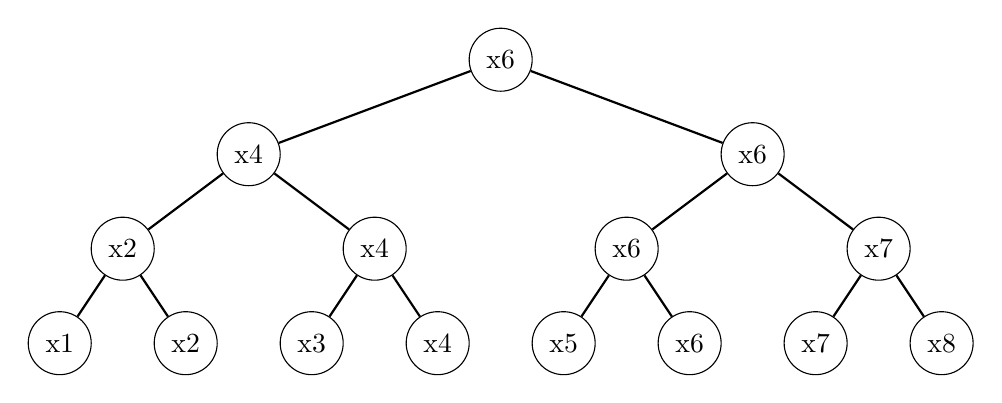
\begin{tikzpicture}[scale=0.8,place/.style={circle,draw, fill=white,inner sep=0pt,minimum size=8mm}]
    \node (x1)  at (0,0) [place] {x1};
    \node (x2)  at (2,0) [place] {x2};
    \node (x3)  at (4,0) [place] {x3};
    \node (x4)  at (6,0) [place] {x4};
    \node (x5)  at (8,0) [place] {x5};
    \node (x6)  at (10,0) [place] {x6};
    \node (x7)  at (12,0) [place] {x7};
    \node (x8)  at (14,0) [place] {x8};
    \node (x21)  at (1,1.5) [place] {x2};
    \node (x22)  at (5,1.5) [place] {x4};
    \node (x23)  at (9,1.5) [place] {x6};
    \node (x24)  at (13,1.5) [place] {x7};
    \node (x31)  at (3,3) [place] {x4};
    \node (x32)  at (11,3) [place] {x6};
    \node (x41)  at (7,4.5) [place] {x6};
    \draw [thick] (x41) -- (x31);
    \draw [thick] (x41) -- (x32);
    \draw [thick] (x31) -- (x21);
    \draw [thick] (x31) -- (x22);
    \draw [thick] (x32) -- (x23);
    \draw [thick] (x32) -- (x24);
    \draw [thick] (x21) -- (x1);
    \draw [thick] (x21) -- (x2);
    \draw [thick] (x22) -- (x3);
    \draw [thick] (x22) -- (x4);
    \draw [thick] (x23) -- (x5);
    \draw [thick] (x23) -- (x6);
    \draw [thick] (x24) -- (x7);
    \draw [thick] (x24) -- (x8);
    \end{tikzpicture}
    \caption{锦标赛的例子;max=x6;次大元素可能是x4,x5,x7}
    \label{Fig:ChampionshipExample01}
\end{figure*}

锦标赛方法之所以叫这个名字是因为它以锦标赛的方法执行比较。关键字分对,“分轮”
比较,胜者进入下一轮。(如果有一轮的关键字数量是奇数,他们中有一个简单的等着
进入下一轮。)锦标赛可以描述成图\ref{Fig:ChampionshipExample01}中显示的二叉树。
每一个叶子包含一个关键字,而每一层的父层都是这一层胜出的胜者。根包含最大的
元素。同算法\ref{Algo:FindMaxValue}一样,需要n-1次比较找到max。

在查找max的过程中,除了max之外的每一个关键字都失败一次。有多少直接失败与max?
如果n是2的整数次幂,这里有$\lg n$轮;一般情况下是$\lceil \lg n\rceil$。既然
每一轮中都有max在,则最多有$\lceil \lg n\rceil$个元素仅失败于max。他们是
secondLargest所有可能的候选。算法\ref{Algo:FindMaxValue}可以用与在$\lceil \lg n\rceil$个
元素中查找最大的,需要做$\lceil \lg n\rceil-1$次比较。因此最坏情况下锦标赛
查找max和secondLargest共需要$n+\lceil \lg n\rceil-2$次比较。这比2n-3是一个进步。
我们可以更好吗?

\subsection{An Adversary Lowe-Bound Argument}
我们考虑的两个方法都是首先找到最大的元素。这不是浪费。任何查找secondLargest
的算法必须也找到max,因为为了知道这个关键字是次大的,首先必须知道它不是
最大的;就是说它必须有一次比较失败。在secondLargest必须失败的那次比较中
胜出的那个就是max。

\subsection{查找max和secondLargest锦标赛方法的实现}
为了找到max进行的锦标赛我们需要一种方法保存每一轮的胜者。在通过锦标赛找到max
之后,只有这些关键字参与查找secondLargest。在我们还不知道那一个是max的时候
我们如何保存那些只败于max的关键字呢?既然锦标赛的概念就是一棵二叉树,自然
的想到了4.8.1小节的\emph{堆结构}。对于n个元素的集合,需要一个有2n-1个节点的
堆结构;就是$E[1], \cdots,E[2*n-1]$。一开始,将元素放在位置$n, \cdots, 2n-1$。
随着锦标赛的过程,将逐步用胜者填写$1, \cdots,n-1$(反着填)。练习5.4显示了
额外的细节。这个算法使用线型的额外空间,运行时间也是线型的。

\section{Selection问题}
假设我们想找到一个数组E中n个元素的中间的元素(我们想元素有rank$\lceil
n/2
\rceil$)。在前面的小节中,我们找到了有效的方法找到rank接近一端或是另一端
(比如最大,最小,同时最大最小,次大的)的方法。练习探索了很多变种,但是
所有的解决这些问题的技术在我们不是对付一端的情况时都将失去效率,对于查找
median都没有用。如果我们找到一个解决方案可以有效的简单排序整个集合,则需要
新的思想。


\subsection{一个分而治之接近}
假设我们能将关键字分成两个集合,$S_1$和$S_2$,这样所有在$S_1$
中的关键字都小于$S_2$ 中的关键字。则

\section{查找median的低限}
我们假设有n个元素的集合E且n是奇数。我们将
\section{Designing Against an Adversary}
设计一个对手可能是一种强大的技术
